\section{Advantages and disadvantages of CBF}\label{sec:cbf_advantages_disadvantages}
Content-based filtering is a powerful approach in recommendation systems, used in many platforms in different contexts. CBF stands in contrast to Collaborative filtering, which uses the other users' interactions to recommend items. While content-based filtering provides some benefits, it also has several limitations.

\subsection{Advantages}
Firstly, Content-based filtering is scalable to a large number of customers, because the user-item matrix is separated for each user. Therefore, by adding new users we shouldn't consider other users' interactions \cite{CBF_Advantages}.

Additionally, CBF can recommend unpopular items if the user has specific preferences. Due to this, Content-based filtering provides capability to recommend new items immediately after publishing them to the platform \cite{CBF_Advantages}.

\subsection{Limitations}
The most crucial problem of CBF is the “cold-start” of recommendations. If the user has zero or small amount of interactions, Content-based filtering couldn't provide preferable data. This limitation cannot be overcome without using Hybrid recommendation systems. Additionally, due to this disadvantage, it is hard to generate recommendations to not-active users, because they have a small amount of interactions \cite{CBF_Disadvantages}.

The other problem relates to recommendation of new content. Content-based filtering won't recommend new content if the user already has a large number of interactions with the other content \cite{CBF_Disadvantages}.

\subsection{Hybrid systems}
Due to some crucial disadvantages of Content-based filtering and other recommendation systems, advanced platforms use hybrid recommendation systems. They are the combination of existing methods and due to that they reduce the impact of disadvantages of each method and improve overall efficiency of the recommendation system\cite{Hybrid_recom_systems}. The diagram of the hybrid system is illustrated in Figure \ref{fig:hybrid_system}.

\begin{figure}
    \centering
    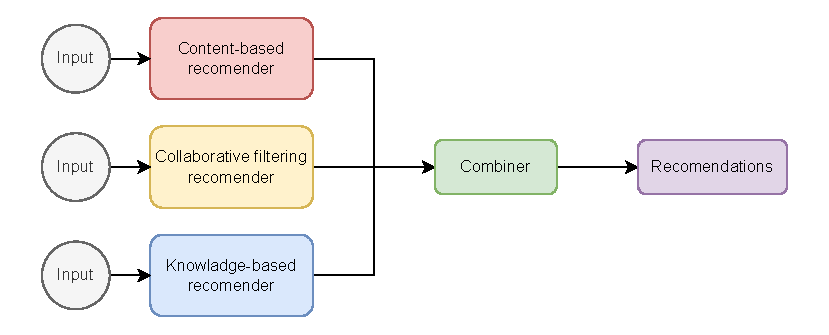
\includegraphics[width=0.6\textwidth]{figures/diagrams/hybrid_systems.pdf}
    \caption{Hybrid recommendation system}
    \label{fig:hybrid_system}
\end{figure}